\documentclass[12pt,a4paper]{article}
\usepackage{pgf}
% \usepackage[condensed,math]{kurier}
% \usepackage[T1]{fontenc}
\usepackage{svg}
\usepackage{tikz}
\usepackage{stanli}
\usepackage{afterpage}
\usepackage{multirow}
\usepackage{subfig}
\usepackage{pgfpages}
\usepackage{svg}
\usepackage{rotating}

%\usepackage{times}


\pgfpagesdeclarelayout{boxed}
{
	\edef\pgfpageoptionborder{0pt}
}
{
	\pgfpagesphysicalpageoptions
	{%
		logical pages=1,%
	}
	\pgfpageslogicalpageoptions{1}
	{
		border code=\pgfsetlinewidth{2pt}\pgfstroke,%
		border shrink=\pgfpageoptionborder,%
		resized width=.9\pgfphysicalwidth,%
		resized height=.9\pgfphysicalheight,%
		center=\pgfpoint{.5\pgfphysicalwidth}{.5\pgfphysicalheight}%
	}%
}

\pgfpagesuselayout{boxed}


% Language setting
% Replace `english' with e.g. `spanish' to change the document language
\usepackage[english]{babel}

% Set page size and margins
% Replace `letterpaper' with `a4paper' for UK/EU standard size
\usepackage[a4paper,top=2cm,bottom=1.5cm,left=1.5cm,right=1.5cm,marginparwidth=1.75cm]{geometry}

% Useful packages
\usepackage{amsmath}
\usepackage{graphicx}
\usepackage[colorlinks=true, allcolors=blue]{hyperref}

\title{}
\author{}
\date{}

\begin{document}
	
	\newcommand{\subf}[2]{%
		{\small\begin{tabular}[t]{@{}c@{}}
				#1\\#2
		\end{tabular}}%
	}
	
	\begin{titlepage}
		\begin{center}
			
			\textbf{}
            
\includegraphics[width=1\textwidth]{utt.png}

            \vspace*{3cm}

			\vspace{1.5cm}
			
			\Huge
			\textbf{Caching strategies for Progressive Web Applications}
			
			\vspace{0.8cm}
			\large
			
			\vspace{0.5cm}
			\LARGE
			
			
			\vfill
			
			
			
			\vspace{0.8cm}
			
			
			
			\Large
			
			
			
			
		\end{center}
		\Large
		\begin{tabbing}
			\hspace*{1em}\= \hspace*{8em} \= \kill % set the tabbings
			\> Name:\>  \textbf{López Bautista Cristian Alexis} \\
			\> Group:\>  10-B \\
			\> Subject:\>  Progressive Web Applications  \\
			\> Professor:  \> Dr. Ray Brunet Parra Galaviz \\
			\> Date: \>  Friday, March 15th, 2024
		\end{tabbing}
		
	\end{titlepage}
	
	
	
	\section{Introduction}

    \paragraph{Caching is one of the most exciting features of SWs. It enables us to deliver to our users a responsive, stable, and native-app-like experience. A web app can display some content and perform some function in bad network conditions, and even when the user is completely offline.}
    
    \paragraph{There are strategies we can use with service workers to respond to “fetch” events. These determine how the service worker will respond to a fetch event based on the type of event request.}
    
    \paragraph{This document will cover five different caching strategies, and describe how and when you should implement each of them:}

    \begin{enumerate}
    
        \item Cache first, Network fallback.
        \item The network first, Cache fallback.
        \item Stale while revalidate
        \item Network only
        \item Cache only
      
    \end{enumerate}

    \section{When to cache resources}

    \paragraph{A PWA can cache resources at any time, but in practice there are a few times when most PWAs will choose to cache them:}

    \subsection{In the service worker's install event handler (precaching)}

    \paragraph{When a service worker is installed, the browser fires an event called install in the service worker's global scope. At this point the service worker can precache resources, fetching them from the network and storing them in the cache. }
    
    \subsection{In the service worker's fetch event handler}

    \paragraph{When a service worker's fetch event fires, the service worker may forward the request to the network and cache the resulting response, either if the cache did not already contain a response, or to update the cached response with a more recent one.}
    
    \subsection{In response to a user request}

    \paragraph{A PWA might explicitly invite the user to download a resource to use later, when the device might be offline. For example, a music player might invite the user to download tracks to play later. In this case the main app thread could fetch the resource and add the response to the cache. Especially if the requested resource is big, the PWA might use the Background Fetch API, and in this case the response will be handled by the service worker, which will add it to the cache.}
    
    \subsection{Periodically}

    \paragraph{Using the Periodic Background Sync API, a service worker might fetch resources periodically and cache the responses, to ensure that the PWA can serve reasonably fresh responses even while the device is offline.}

    \section{Caching strategies}

    \subsection{Cache first, Network fallback.}

    \paragraph{The service worker will loads the local (cached) assets (HTML, CSS, images, fonts, etc.), if possible, bypassing the network. If cached content is not available, the service worker returns a response from the web instead and caches the network response. This strategy can be used when dealing with remote resources that are very unlikely to change, such as static images.}

    \begin{figure}[h!]
      \centering
      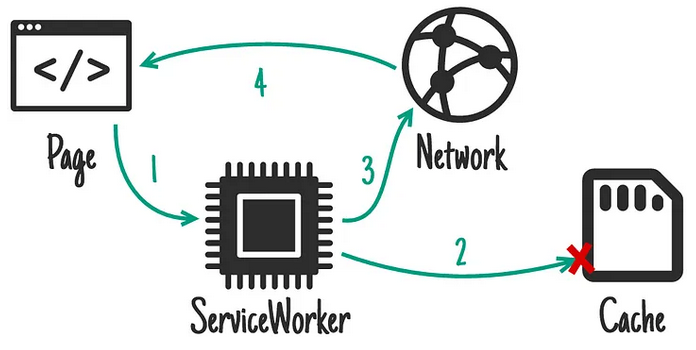
\includegraphics[width=0.5\textwidth]{cachefirst.png}
      \caption{Cache first strategy.}
    \end{figure}

    \subsection{The network first, Cache fallback.}

    \paragraph{In this strategy, the service worker will check the network first for a response and, if successful, returns current data to the page. If the network request fails, then the service worker returns the cached entry instead. Use this when data must be as fresh as possible, such as a real-time API response, but you still want to display something as a fallback when the network is unavailable.}

    \begin{figure}[h!]
      \centering
      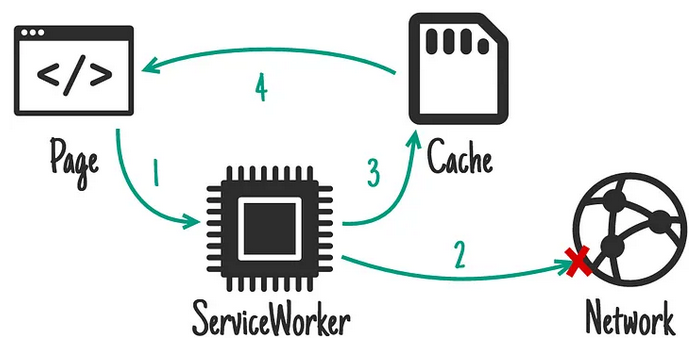
\includegraphics[width=0.5\textwidth]{networkfirst.png}
      \caption{Network first strategy.}
    \end{figure}

    \subsection{Stale while revalidate}

    \paragraph{The stale-while-revalidate pattern allows you to respond to the request as quickly as possible with a cached response if available, falling back to the network request if it’s not cached. The network request is then used to update the cache. This is a fairly common strategy where having the most up-to-date resource is not vital to the application.}

    \begin{figure}[h!]
      \centering
      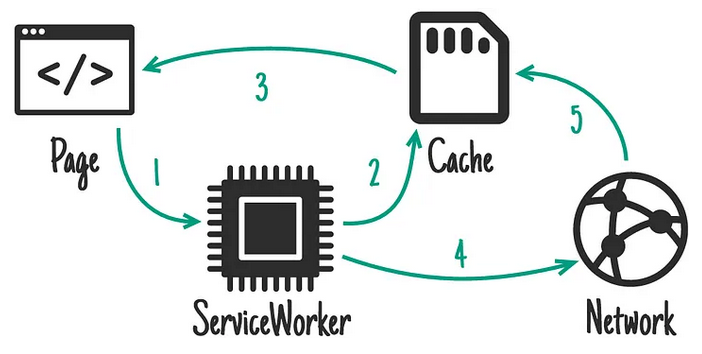
\includegraphics[width=0.5\textwidth]{stale.png}
      \caption{Stale strategy.}
    \end{figure}

    \subsection{Network only}

    \paragraph{In this, the service worker will only check the network. There is no going to the cache for data. If the network fails, then the request fails. This can be used when only fresh data can be displayed on your site.}

    \begin{figure}[h!]
      \centering
      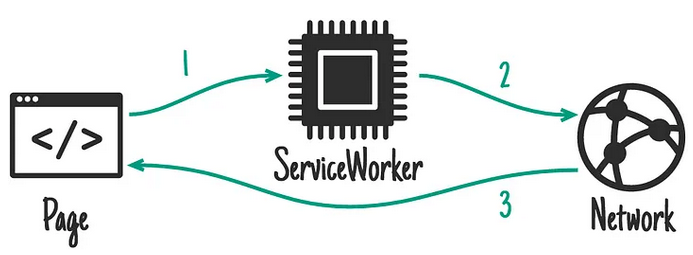
\includegraphics[width=0.5\textwidth]{networkonly.png}
      \caption{Network only strategy.}
    \end{figure}

    \subsection{Cache only}

    \paragraph{The data is cached during the install event so that you can depend on the information being there. This can be useful if you have your own precaching step.}

    \begin{figure}[h!]
      \centering
      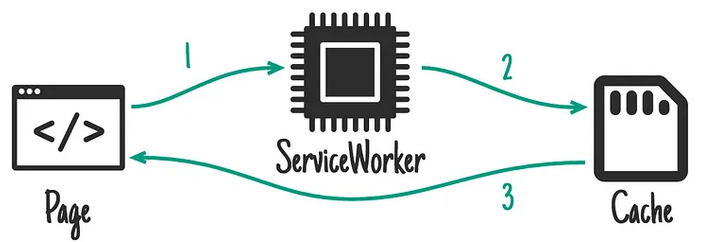
\includegraphics[width=0.5\textwidth]{cacheonly.png}
      \caption{Cache only strategy.}
    \end{figure}

    \section{Examples}

    \paragraph{Pre-cache the home page assets when the user lands on the onboarding page through the install event. With this, once the user completes the onboarding, all the static assets needed to load the home page are already available in the cache.}

    \begin{verbatim}
    self.addEventListener(‘install’, async function (event) {
      event.waitUntil(caches.open(‘assets’).then(function (cache) {
        return cache.addAll(filesToCache);
     }));
    });
    \end{verbatim}

    \paragraph{Network-only strategy to handle all navigations. This ensures that the pages are loaded from the network only and fall back to an offline page if the internet is not available.}

    \begin{verbatim}
    var networkOnly = new NetworkOnly();
    var navigationHandler = async function navigationHandler(params) {
      try {
        return await networkOnly.handle(params);
      } catch (error) {
        return caches.match(FALLBACK_HTML_URL, {
          cacheName: 'offline'
        });
      }
    };// Register this strategy to handle all navigations.
    var navigationRoute = new workbox.routing.NavigationRoute(navigationHandler);
    registerRoute(navigationRoute);
    \end{verbatim}

    \paragraph{Stale While Revalidate strategy for CSS and js assets. All the CSS/js assets are loaded from the cache and returns to the user immediately. Same time, it will check for any updates also from the network as well. If the file is updated in the network, the service worker will update the cache. So next time, when the user loads the same page, he will get the updated version.}

    \begin{verbatim}
    registerRoute(function(_ref2) {
    var request = _ref2.request;
    return request.destination === 'style' || request.destination === 'script';
    }, new StaleWhileRevalidate({
        cacheName: 'assets',
        plugins: [new CacheableResponsePlugin({
            statuses: [200]
        })]
    }));
    \end{verbatim}

    \paragraph{Cache First for the images. The images we use are usually not updated on the server frequently. So I’ve used the cache first strategy for loading the static images with few options as well. Since the images can bloat your cache disk quickly, we have put a maximum image limit in the cache with maxEntries. Use purgeOnQuotaError along with this to make sure that the cache is cleared when the quota exceeds. Also, I’ve applied maxAgeSeconds to expire the image cache.}

    \begin{verbatim}
    registerRoute(function(_ref) {
        var request = _ref.request;
        return request.destination === 'image';
    }, new CacheFirst({
        cacheName: 'images',
        plugins: [new CacheableResponsePlugin({
            statuses: [200]
        }), new ExpirationPlugin({
            maxEntries: 50,
            maxAgeSeconds: 60 * 60 * 24 * 30, // 30 Days
            purgeOnQuotaError: true
        })]
    }));
    \end{verbatim}

\clearpage

	\section{Bibliography}

    \begin{enumerate}
    
      \item Babu, L. V. (2021, december 27th). Best Caching strategies — Progressive Web App (PWA). Medium. 
      
      \href{https://medium.com/animall-engineering/best-caching-strategies-progressive-web-app-pwa-c610d65b2009}{https://medium.com/animall-engineering/best-caching-strategies-progressive-web-app-pwa-c610d65b2009}

       \item Caching - Progressive web apps | MDN. (2023, october 25th). MDN Web Docs. 
      
      \href{https://developer.mozilla.org/en-US/docs/Web/Progressive_web_apps/Guides/Caching}{https://developer.mozilla.org/en-US/docs/Web/Progressive_web_apps/Guides/Caching}

      \item Educative. (s. f.). Educative Answers - Trusted Answers to Developer Questions.
      
      \href{https://www.educative.io/answers/5-service-worker-caching-strategies-for-your-next-pwa-app}{https://www.educative.io/answers/5-service-worker-caching-strategies-for-your-next-pwa-app}
      
    \end{enumerate}
	
	
\end{document}